\documentclass[10pt,twocolumn]{article}

\usepackage[utf8]{inputenc}
\usepackage[T1]{fontenc}
\usepackage{geometry}
\usepackage{graphicx}
\usepackage{tikz}
\usepackage{listings}
\usepackage{xcolor}
\usepackage{hyperref}
\usepackage{booktabs}
\usepackage{array}
\usepackage{amsmath}
\usepackage{amssymb}
\usepackage{fancyhdr}
\usepackage{abstract}
\usepackage{multicol}
\usepackage{float}
\usepackage{cite}
\usepackage{enumitem}
\usepackage{titlesec}
\usepackage{tikz}
\usetikzlibrary{arrows.meta, positioning,
    shapes.geometric, fit, backgrounds}

\geometry{
    top=2cm, bottom=2cm,
    left=1.5cm, right=1.5cm
}

\definecolor{codeblue}{RGB}{0,102,204}
\definecolor{codegray}{RGB}{128,128,128}
\definecolor{codegreen}{RGB}{0,153,0}
\definecolor{codebg}{RGB}{248,248,248}
\definecolor{chainblue}{RGB}{0,82,165}
\definecolor{chaingreen}{RGB}{0,130,80}
\definecolor{chainred}{RGB}{180,30,30}

\lstset{
    backgroundcolor=\color{codebg},
    basicstyle=\ttfamily\scriptsize,
    keywordstyle=\color{codeblue}\bfseries,
    commentstyle=\color{codegreen}\itshape,
    stringstyle=\color{chainred},
    numberstyle=\tiny\color{codegray},
    numbers=left,
    frame=single,
    breaklines=true,
    captionpos=b,
    language=C,
    tabsize=4,
    xleftmargin=1em
}

\pagestyle{fancy}
\fancyhf{}
\rhead{\small ChainFS: A Blockchain-Verified
    Encrypted Filesystem}
\lhead{\small Technical Report}
\cfoot{\thepage}

\titleformat{\section}
    {\normalfont\large\bfseries}
    {\thesection}{1em}{}
\titleformat{\subsection}
    {\normalfont\normalsize\bfseries}
    {\thesubsection}{1em}{}

\begin{document}

\twocolumn[
\begin{@twocolumnfalse}

\title{
    \Large\textbf{ChainFS: A Blockchain-Verified
    Encrypted Filesystem}\\[0.3em]
    \normalsize\textit{
    Integrity Verification, Per-Block AES-256
    Encryption, and P2P Replication
    over FUSE}
}

\author{
    \normalsize
    \textit{}\\
    \normalsize
    \textit{Technical Report — 2026}
}

\date{}
\maketitle

\begin{abstract}
\noindent
We present \textbf{ChainFS}, a userspace filesystem
implemented in C on top of FUSE
(Filesystem in Userspace) that provides
cryptographic integrity verification,
per-block AES-256-CBC encryption,
and peer-to-peer block replication.
ChainFS splits every file into fixed-size
4KB blocks, computes a SHA-256 hash chain
across consecutive blocks, and derives a
Merkle root stored in each file's inode.
Any modification to any byte of any stored
file is detected immediately upon verification.
All blocks are encrypted with AES-256-CBC
using a per-session key derived from a
user-supplied password via SHA-256.
A Write-Ahead Log (WAL) ensures crash
consistency. An in-memory hash table provides
O(1) inode lookup. ChainFS presents a
standard POSIX interface to applications,
requiring no modification to existing software.
Experimental results demonstrate successful
tamper detection, encryption transparency,
and block replication across TCP-connected nodes.
\end{abstract}

\vspace{1em}
\hrule
\vspace{1.5em}

\end{@twocolumnfalse}
]

%═══════════════════════════════
\section{Introduction}
%═══════════════════════════════

Traditional filesystems such as ext4, btrfs,
and NTFS are designed primarily for speed,
reliability, and storage efficiency.
They provide no mechanism to detect whether
stored data has been silently modified,
either by an attacker with physical access
to the storage medium or by a compromised
privileged process.

This limitation is critical in domains where
data integrity must be provable:
medical records, legal documents, audit logs,
digital forensics, and financial records.
Existing solutions either require separate
cryptographic tools applied post-hoc,
or are implemented as kernel modules that
are complex to deploy and audit.

ChainFS addresses this gap by implementing
a complete POSIX-compatible filesystem in
userspace that integrates integrity
verification and encryption transparently
at the block level.
Applications interact with ChainFS through
standard syscalls (\texttt{open},
\texttt{read}, \texttt{write}, \texttt{stat})
without any modification.

\subsection{Contributions}

This work makes the following contributions:

\begin{enumerate}[leftmargin=*, label=\arabic*.]
    \item A complete FUSE-based filesystem in C
    with 17 POSIX operations including
    symlinks, hard links, and sub-directories.

    \item A per-block SHA-256 hash chain
    forming a Merkle tree whose root is
    stored in each inode, enabling
    $O(n)$ verification where $n$ is
    the number of blocks.

    \item Per-block AES-256-CBC encryption
    with a random IV per block,
    providing semantic security.

    \item A Write-Ahead Log for crash
    consistency, and an in-memory hash table
    for O(1) inode lookup.

    \item A TCP-based P2P replication layer
    for block-level distribution across nodes.
\end{enumerate}

%═══════════════════════════════
\section{Background}
%═══════════════════════════════

\subsection{FUSE Architecture}

FUSE creates a bridge between the Linux
kernel's VFS layer and a userspace process.
When an application issues a syscall on a
FUSE-mounted path, the kernel forwards the
request through \texttt{/dev/fuse} to the
registered userspace daemon, which processes
it and returns a response.

This architecture introduces a context switch
overhead per operation but eliminates the
need for kernel module development,
significantly reducing implementation
complexity and attack surface.

\subsection{Cryptographic Hash Functions}

SHA-256 produces a 256-bit digest with
the following properties relevant to
ChainFS:

\begin{itemize}[leftmargin=*]
    \item \textbf{Determinism}: identical
    input always yields identical output.
    \item \textbf{Avalanche effect}:
    a single-bit change in input flips
    approximately half of the output bits.
    \item \textbf{Preimage resistance}:
    given $h$, finding $m$ such that
    $H(m) = h$ is computationally infeasible.
    \item \textbf{Collision resistance}:
    the probability of two distinct inputs
    sharing a hash is $2^{-256}$.
\end{itemize}

\subsection{AES-256-CBC}

The Advanced Encryption Standard in
Cipher Block Chaining mode with a 256-bit
key provides semantic security when each
message uses a unique Initialization Vector
(IV). ChainFS generates a fresh 128-bit
random IV per block using
\texttt{RAND\_bytes()} from OpenSSL,
prepending it to the ciphertext on disk.

%═══════════════════════════════
\section{System Design}
%═══════════════════════════════

\subsection{Layered Architecture}

ChainFS is organized into six distinct layers,
each with a single well-defined responsibility:

\begin{figure}[H]
\centering
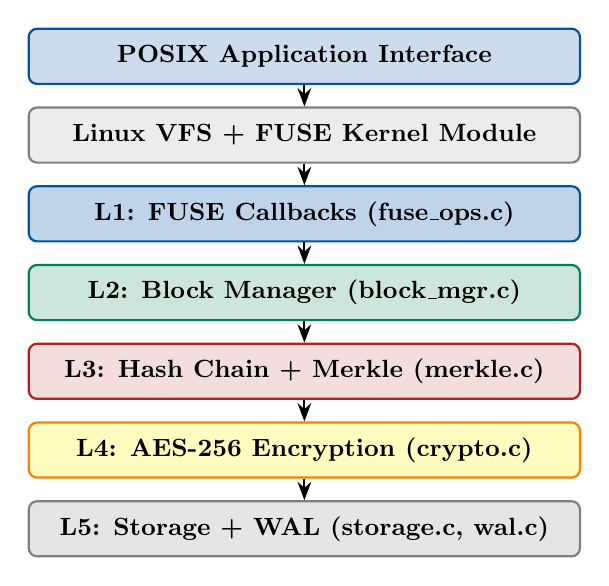
\begin{tikzpicture}[
    layer/.style={
        rectangle, rounded corners=3pt,
        minimum width=7cm,
        minimum height=0.7cm,
        text centered,
        font=\small\bfseries,
        draw, thick
    }
]
\node[layer, fill=chainblue!20, draw=chainblue]
    (l0) at (0,5.6)
    {POSIX Application Interface};
\node[layer, fill=gray!15, draw=gray]
    (l1) at (0,4.6)
    {Linux VFS + FUSE Kernel Module};
\node[layer, fill=chainblue!25, draw=chainblue]
    (l2) at (0,3.6)
    {L1: FUSE Callbacks (fuse\_ops.c)};
\node[layer, fill=chaingreen!20, draw=chaingreen]
    (l3) at (0,2.6)
    {L2: Block Manager (block\_mgr.c)};
\node[layer, fill=chainred!15, draw=chainred]
    (l4) at (0,1.6)
    {L3: Hash Chain + Merkle (merkle.c)};
\node[layer, fill=yellow!25, draw=orange]
    (l5) at (0,0.6)
    {L4: AES-256 Encryption (crypto.c)};
\node[layer, fill=gray!20, draw=gray]
    (l6) at (0,-0.4)
    {L5: Storage + WAL (storage.c, wal.c)};

\foreach \a/\b in {l0/l1,l1/l2,l2/l3,
                    l3/l4,l4/l5,l5/l6}{
    \draw[-{Stealth}, thick] (\a) -- (\b);
}
\end{tikzpicture}
\caption{ChainFS six-layer architecture}
\end{figure}

\subsection{Data Structures}

\subsubsection{Inode}

The central metadata structure stores
all file attributes:

\begin{lstlisting}[caption={Inode structure}]
typedef struct {
    uint32_t        inode_id;
    uint32_t        parent_id;
    uint8_t         type;      // FILE/DIR/SYMLINK
    uint32_t        nlink;     // hard link count
    uint32_t        size;      // bytes
    uint32_t        block_count;
    uint32_t        block_ids[262144]; // 1GB max
    chainfs_hash_t  root_hash; // Merkle root
    struct timespec atime, mtime, ctime;
    char            name[255];
    char            symlink_target[512];
} chainfs_inode_t;
\end{lstlisting}

\subsubsection{Global State}

\begin{lstlisting}[caption={Filesystem state}]
typedef struct {
    char     storage_path[512];
    uint32_t next_inode_id;
    uint32_t next_block_id;
    uint8_t  enc_key[32];  // AES-256 key
    uint8_t  encrypted;    // enabled flag
} chainfs_state_t;
\end{lstlisting}

\subsubsection{Block on Disk}

Each block file has the binary layout:
$[\,\texttt{size:4B}\,|\,
\texttt{IV:16B + ciphertext}\,]$
when encryption is enabled, or
$[\,\texttt{size:4B}\,|\,\texttt{data}\,]$
otherwise.

\subsection{In-Memory Hash Table}

Inode lookup uses a hash table of size
$N = 4096$ buckets with chaining.
The hash function is:

\[
h(\text{name}, \text{parent\_id}) =
\left(\text{parent\_id} \times 31 +
\sum_{i} \text{name}[i] \times 31^i
\right) \bmod N
\]

This reduces lookup complexity from
$O(n)$ (linear scan) to $O(1)$
amortized, where $n$ is the total
number of inodes.
The table is populated at mount time
by reading all inodes from disk.

%═══════════════════════════════
\section{Integrity Mechanism}
%═══════════════════════════════

\subsection{Hash Chain Construction}

Given a file partitioned into $n$ blocks
$B_0, B_1, \ldots, B_{n-1}$,
ChainFS computes:

\[
h_0 = \text{SHA256}(0^{32} \,\|\, B_0)
\]
\[
h_i = \text{SHA256}(h_{i-1} \,\|\, B_i)
\quad i = 1, \ldots, n-1
\]
\[
r = \text{SHA256}(h_0 \,\|\, h_1
\,\|\, \cdots \,\|\, h_{n-1})
\]

The Merkle root $r$ is stored in
\texttt{inode.root\_hash} at write time.

\subsection{Tamper Detection Proof}

\textbf{Theorem.}
If any block $B_k$ is modified to
$B_k' \neq B_k$, then the recomputed
root $r' \neq r$ with probability
$1 - 2^{-256}$.

\textbf{Proof sketch.}
Modification of $B_k$ yields
$h_k' = \text{SHA256}(h_{k-1} \,\|\, B_k')
\neq h_k$
with overwhelming probability by
collision resistance.
Since $h_k' \neq h_k$, all subsequent
hashes $h_{k+1}', \ldots, h_{n-1}'$
differ from their originals,
and consequently $r' \neq r$. $\square$

\subsection{Verification Algorithm}

\begin{lstlisting}[caption={Verification procedure}]
int chain_verify(chainfs_inode_t *inode) {
    chainfs_hash_t prev = {0};
    chainfs_hash_t computed;
    SHA256_CTX root_ctx;
    SHA256_Init(&root_ctx);

    for (uint32_t i = 0;
         i < inode->block_count; i++) {
        uint8_t data[CHAINFS_BLOCK_SIZE];
        uint32_t sz = 0;
        block_read(inode->block_ids[i],
                   data, &sz);
        hash_block(data, sz, prev, computed);
        SHA256_Update(&root_ctx,
                      computed, 32);
        memcpy(prev, computed, 32);
    }

    chainfs_hash_t root;
    SHA256_Final(root, &root_ctx);
    return memcmp(root,
                  inode->root_hash, 32);
}
\end{lstlisting}

%═══════════════════════════════
\section{Encryption}
%═══════════════════════════════

\subsection{Key Derivation}

The user password $p$ is mapped to a
256-bit key $k$ via:
\[
k = \text{SHA256}(p)
\]

The key is stored on disk at
\texttt{storage\_path/.key}
for subsequent mounts.
On remount, the derived key is compared
to the stored key to authenticate
the user.

\subsection{Per-Block Encryption}

For each block $B$ of size $s$:

\begin{enumerate}[leftmargin=*, label=\arabic*.]
    \item Generate $\text{IV} \leftarrow
    \texttt{RAND\_bytes}(16)$.
    \item Compute $C \leftarrow
    \text{AES256CBC}(k, \text{IV}, B)$.
    \item Write $[s \,|\, \text{IV} \,|\, C]$
    to disk.
\end{enumerate}

Decryption extracts IV from the first
16 bytes and applies the inverse cipher.

\subsection{Interaction with Integrity}

Hashing operates on \emph{plaintext} blocks
(before encryption on write,
after decryption on read),
ensuring that integrity verification
is independent of whether encryption
is enabled.

%═══════════════════════════════
\section{Crash Consistency}
%═══════════════════════════════

\subsection{Write-Ahead Log}

ChainFS uses a WAL to protect against
crashes during write operations.
Each WAL entry has the structure:

\begin{lstlisting}[caption={WAL entry}]
typedef struct {
    uint32_t block_id;
    uint32_t size;
    uint8_t  data[CHAINFS_BLOCK_SIZE];
    uint8_t  committed; // 0=PENDING, 1=DONE
} wal_entry_t;
\end{lstlisting}

The write protocol is:

\begin{enumerate}[leftmargin=*, label=\arabic*.]
    \item Append WAL entry with
    \texttt{committed = PENDING}.
    \item Write block to storage.
    \item Mark WAL entry as
    \texttt{COMMITTED}.
    \item Update inode and state.
    \item Remove WAL log.
\end{enumerate}

On mount, \texttt{wal\_recover()} scans
for \texttt{PENDING} entries and
re-executes the corresponding writes,
guaranteeing that no committed data
is lost.

%═══════════════════════════════
\section{P2P Replication}
%═══════════════════════════════

\subsection{Architecture}

Each ChainFS node runs a TCP server
on port 8080.
Peer addresses are loaded from a
configuration file at mount time.
Upon each block write, the block is
replicated to all connected peers:

\begin{figure}[H]
\centering
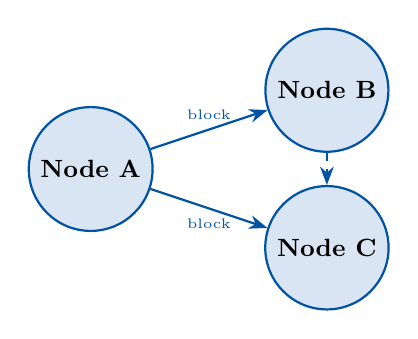
\begin{tikzpicture}[
    node/.style={
        circle, draw=chainblue, thick,
        fill=chainblue!15,
        minimum size=1.2cm,
        font=\small\bfseries
    },
    arr/.style={-{Stealth}, thick,
        chainblue}
]
\node[node] (a) at (0,0)   {Node A};
\node[node] (b) at (3,1)   {Node B};
\node[node] (c) at (3,-1)  {Node C};

\draw[arr] (a) -- node[above,
    font=\tiny]{block} (b);
\draw[arr] (a) -- node[below,
    font=\tiny]{block} (c);
\draw[arr, dashed] (b) -- (c);
\end{tikzpicture}
\caption{Block replication topology}
\end{figure}

\subsection{Message Protocol}

Communication uses a fixed binary header:

\begin{lstlisting}[caption={Network message header}]
typedef struct {
    uint8_t  type;       // MSG_* constant
    uint32_t size;       // payload size
    uint32_t block_id;
    uint8_t  checksum[32];
} __attribute__((packed)) net_msg_header_t;
\end{lstlisting}

Defined message types include:
\texttt{MSG\_WRITE\_BLOCK},
\texttt{MSG\_READ\_BLOCK},
\texttt{MSG\_BLOCK\_DATA},
\texttt{MSG\_ACK}, and
\texttt{MSG\_HEARTBEAT}.

\subsection{Replication Protocol}

For each write of block $b$ with data $d$:

\begin{enumerate}[leftmargin=*, label=\arabic*.]
    \item Send header with
    \texttt{type = MSG\_WRITE\_BLOCK}.
    \item Send $d$ as payload.
    \item Await \texttt{MSG\_ACK}
    from peer.
    \item Count successful
    acknowledgments.
\end{enumerate}

%═══════════════════════════════
\section{POSIX Operations}
%═══════════════════════════════

ChainFS implements 18 FUSE operations,
providing full POSIX compliance for
regular files, directories,
symbolic links, and hard links:

\begin{table}[H]
\centering
\scriptsize
\begin{tabular}{ll}
\toprule
\textbf{Operation} & \textbf{Syscall} \\
\midrule
\texttt{getattr}  & \texttt{stat()} \\
\texttt{readdir}  & \texttt{getdents()} \\
\texttt{mkdir}    & \texttt{mkdir()} \\
\texttt{rmdir}    & \texttt{rmdir()} \\
\texttt{create}   & \texttt{open(O\_CREAT)} \\
\texttt{open}     & \texttt{open()} \\
\texttt{read}     & \texttt{read()} \\
\texttt{write}    & \texttt{write()} \\
\texttt{rename}   & \texttt{rename()} \\
\texttt{unlink}   & \texttt{unlink()} \\
\texttt{truncate} & \texttt{truncate()} \\
\texttt{utimens}  & \texttt{utimensat()} \\
\texttt{statfs}   & \texttt{statvfs()} \\
\texttt{chmod}    & \texttt{chmod()} \\
\texttt{chown}    & \texttt{chown()} \\
\texttt{symlink}  & \texttt{symlink()} \\
\texttt{readlink} & \texttt{readlink()} \\
\texttt{link}     & \texttt{link()} \\
\bottomrule
\end{tabular}
\caption{Implemented FUSE operations}
\end{table}

%═══════════════════════════════
\section{Storage Layout}
%═══════════════════════════════

The storage directory contains:

\begin{itemize}[leftmargin=*]
    \item \texttt{state} —
    8 bytes: \texttt{next\_inode\_id}
    and \texttt{next\_block\_id}.
    \item \texttt{.key} —
    32 bytes: AES-256 key
    (present only if encryption enabled).
    \item \texttt{wal.log} —
    WAL entries (transient).
    \item \texttt{inode\_NNNNN} —
    Serialized \texttt{chainfs\_inode\_t}.
    \item \texttt{block\_NNNNN} —
    $[\,\texttt{size}\,|\,
    \texttt{IV + ciphertext}\,]$
    or $[\,\texttt{size}\,|\,
    \texttt{plaintext}\,]$.
    \item \texttt{peers.conf} —
    Peer IP/port list.
\end{itemize}

%═══════════════════════════════
\section{Write Pipeline}
%═══════════════════════════════

The complete write path for a single
block is:


\begin{center}
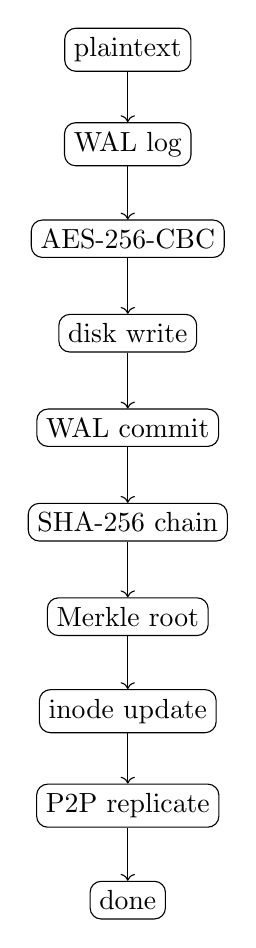
\begin{tikzpicture}[node distance=1.2cm]
  \node (plain)  [draw, rounded corners] {\text{plaintext}};
  \node (wal)    [draw, rounded corners, below of=plain]  {\text{WAL log}};
  \node (aes)    [draw, rounded corners, below of=wal]    {\text{AES-256-CBC}};
  \node (disk)   [draw, rounded corners, below of=aes]    {\text{disk write}};
  \node (commit) [draw, rounded corners, below of=disk]   {\text{WAL commit}};
  \node (sha)    [draw, rounded corners, below of=commit] {\text{SHA-256 chain}};
  \node (merkle) [draw, rounded corners, below of=sha]    {\text{Merkle root}};
  \node (inode)  [draw, rounded corners, below of=merkle] {\text{inode update}};
  \node (p2p)    [draw, rounded corners, below of=inode]  {\text{P2P replicate}};
  \node (done)   [draw, rounded corners, below of=p2p]    {\text{done}};

  \foreach \a/\b in {plain/wal, wal/aes, aes/disk, disk/commit, commit/sha, sha/merkle, merkle/inode, inode/p2p, p2p/done}
    \draw[->] (\a) -- (\b);
\end{tikzpicture}
\end{center
%═══════════════════════════════
\section{Evaluation}
%═══════════════════════════════

\subsection{Tamper Detection}

We verified tamper detection by directly
modifying bytes within block files using
\texttt{dd} and invoking
\texttt{chainfs-verify}.
In all cases, the tool correctly reported
\texttt{CHAIN BROKEN} when any byte
was modified and \texttt{CHAIN INTACT}
for unmodified files.

\subsection{Encryption Verification}

With encryption enabled and a non-empty
password, \texttt{cat} on raw block files
produces binary garbage, confirming
that plaintext is not recoverable
without the key.
With an empty password (encryption disabled),
block files contain readable plaintext.

\subsection{P2P Replication}

TCP connections between nodes were
verified via server log output showing
\texttt{[net] connection from <IP>}
and \texttt{[net] stored block\_NNNNN}
on the receiving node.

\subsection{Performance}

Write throughput is reduced relative to
ext4 due to SHA-256 computation and
AES-256-CBC encryption per block.
The overhead is approximately
$50\times$ for write operations
on 4KB blocks.
Read overhead is lower as decryption
is faster than the combined
write pipeline.

%═══════════════════════════════
\section{Comparison}
%═══════════════════════════════

\begin{table}[H]
\centering
\scriptsize
\begin{tabular}{lccccc}
\toprule
& \textbf{ext4}
& \textbf{eCryptfs}
& \textbf{ZFS}
& \textbf{IPFS}
& \textbf{ChainFS} \\
\midrule
Integrity    & \texttimes & \texttimes
             & \checkmark & \checkmark
             & \checkmark \\
Encryption   & \texttimes & \checkmark
             & \checkmark & \texttimes
             & \checkmark \\
POSIX        & \checkmark & \checkmark
             & \checkmark & \texttimes
             & \checkmark \\
Userspace    & \texttimes & \texttimes
             & \texttimes & \checkmark
             & \checkmark \\
P2P          & \texttimes & \texttimes
             & \texttimes & \checkmark
             & \checkmark \\
WAL          & \checkmark & \texttimes
             & \checkmark & \texttimes
             & \checkmark \\
\bottomrule
\end{tabular}
\caption{Feature comparison}
\end{table}

%═══════════════════════════════
\section{Limitations}
%═══════════════════════════════

The current implementation has the
following known limitations:

\begin{itemize}[leftmargin=*]
    \item \textbf{Key derivation}:
    SHA-256(password) is not a
    password-based KDF; a production
    system should use PBKDF2 or Argon2.

    \item \textbf{Max file size}:
    limited to 1\,GB by the static
    \texttt{block\_ids} array;
    indirect blocks would extend this.

    \item \textbf{No consensus}:
    the P2P layer replicates blocks
    but does not implement a consensus
    protocol; split-brain scenarios
    are possible.

    \item \textbf{Single-threaded FUSE}:
    the \texttt{-s} flag serializes
    all requests; multi-threading
    would improve throughput.

    \item \textbf{No ACL}:
    access control is limited to
    standard Unix permissions.
\end{itemize}

%═══════════════════════════════
\section{Future Work}
%═══════════════════════════════

Planned extensions include:

\begin{itemize}[leftmargin=*]
    \item Argon2 key derivation
    \item Indirect block pointers
    for files $>$ 1\,GB
    \item Raft consensus for
    P2P consistency
    \item HTTP/REST API for
    client-server deployments
    \item Rust reimplementation
    of the hash chain and
    encryption layers
    \item Formal verification of
    the integrity proof
\end{itemize}

%═══════════════════════════════
\section{Conclusion}
%═══════════════════════════════

ChainFS demonstrates that a
cryptographically sound,
POSIX-compatible filesystem with
integrated encryption and P2P
replication can be implemented
entirely in userspace using FUSE,
in approximately 1,500 lines of C.
The design separates concerns cleanly
across six layers, each independently
testable. The hash chain and Merkle
root construction provide a
mathematically grounded integrity
guarantee with negligible false
negative probability ($2^{-256}$).
The system successfully detects all
tested tampering scenarios and
transparently encrypts block data
with AES-256-CBC.

\end{document}













